%%%%%%%%%%%%%%%%%%%%%%%%%%%%%%%%%%%%%%%%%%%%%%%%%%%%%%%%%%%%%%%%%%%%%%%%%
%%%%%%%%%%%%%%%%%%%%%%%%%%%%%%%%%%%%%%%%%%%%%%%%%%%%%%%%%%%%%%%%%%%%%%%%%
%%%%%%%%%%%%%%%%%%%%%%%%%%%%%%%%%%%%%%%%%%%%%%%%%%%%%%%%%%%%%%%%%%%%%%%%%
% Motivation
%%%%%%%%%%%%%%%%%%%%%%%%%%%%%%%%%%%%%%%%%%%%%%%%%%%%%%%%%%%%%%%%%%%%%%%%%
%%%%%%%%%%%%%%%%%%%%%%%%%%%%%%%%%%%%%%%%%%%%%%%%%%%%%%%%%%%%%%%%%%%%%%%%%
%%%%%%%%%%%%%%%%%%%%%%%%%%%%%%%%%%%%%%%%%%%%%%%%%%%%%%%%%%%%%%%%%%%%%%%%%
\begin{frame}
  \frametitle{Motivation}
  \begin{columns}
    \column{0.53\textwidth}
    \begin{itemize}
      \item Algorithms suffer from \emph{state explosion} when processing \emph{large} automata.\justifying\vspace*{0.5em}
      \item<2-> State-of-the-art minimization methods (\emph{state merging} and \emph{transition pruning}) can leave \emph{redundant substructures} in the resulting automata.\justifying\vspace*{0.5em}
      \item<3-> Smaller automata means \emph{faster} and \emph{cheaper} computations, generally \emph{more efficient} (can be used within hardware for high-speed \emph{network filtering}).\justifying\vspace*{0.5em}
      \item<4-> Why not take inspiration from programming languages and use \emph{procedures} and a \emph{stack} for repetitive substructures?\justifying
    \end{itemize}

    \column{0.45\textwidth}
    \vspace*{-0.8em}
    \begin{figure}
      \centering
      \begin{tikzpicture}[scale=0.6, every node/.style={scale=0.6}, node distance=2cm]
        \node[state, initial above, initial text=start] (0) {$0$};
        \node[cloud, aspect=4, draw, cloud puffs=20, cloud puff arc=90, below left=0.9cm and 0.45cm of 0] (1) {\hspace*{-1.5em}\texttt{.*new XMLHttpRequest}\hspace*{-1.5em}};
        \node[cloud, aspect=4, draw, cloud puffs=10, cloud puff arc=90, below right=0.97cm and 0.805cm of 0] (2) {\texttt{.*file://}};
        \node[state, below left=0.55cm and 1.25cm of 0, fill=orange] (11) {$\textbf{1}$};
        \node[state, below right=0.55cm and 1.25cm of 0, fill=white!50!blue] (22) {$\textbf{2}$};
        \node[state, below=0.4cm of 11, fill=orange] (33) {$\textbf{3}$};
        \node[state, below=0.4cm of 22, fill=white!50!blue] (44) {$\textbf{4}$};
        \node[cloud, aspect=4, draw, cloud puffs=10, cloud puff arc=90, below=1.4cm of 1] (5) {\texttt{.*file://}};
        \node[cloud, aspect=4, draw, cloud puffs=20, cloud puff arc=90, below=1.4cm of 2] (6) {\hspace*{-1.5em}\texttt{.*new XMLHttpRequest}\hspace*{-1.5em}};
        \node[state, below=0.7cm of 33, fill=white!20!red] (55) {$\textbf{5}$};
        \node[state, below=0.7cm of 44, fill=black!20!green] (66) {$\textbf{6}$};
        \node[state, below=0.4 of 55, fill=white!20!red] (77) {$\textbf{7}$};
        \node[state, below=0.4 of 66, fill=black!20!green] (88) {$\textbf{8}$};
        \node[state, accepting, below left=0.55cm and 1.25cm of 88] (9) {$9$};

        \path[->]
                  (0) edge[out=west, in=north] node[above] {$\varepsilon$} (11)
                  (0) edge[out=east, in=north] node[above] {$\varepsilon$} (22)
                  (33) edge node[left] {$\varepsilon$} (55)
                  (44) edge node[right] {$\varepsilon$} (66)
                  (77) edge[out=south, in=west] node[below] {$\varepsilon$} (9)
                  (88) edge[out=south, in=east] node[below] {$\varepsilon$} (9);

      \end{tikzpicture}
    \end{figure}
  \end{columns}
\end{frame}


%%%%%%%%%%%%%%%%%%%%%%%%%%%%%%%%%%%%%%%%%%%%%%%%%%%%%%%%%%%%%%%%%%%%%%%%%
%%%%%%%%%%%%%%%%%%%%%%%%%%%%%%%%%%%%%%%%%%%%%%%%%%%%%%%%%%%%%%%%%%%%%%%%%
%%%%%%%%%%%%%%%%%%%%%%%%%%%%%%%%%%%%%%%%%%%%%%%%%%%%%%%%%%%%%%%%%%%%%%%%%
% Procedure Finding
%%%%%%%%%%%%%%%%%%%%%%%%%%%%%%%%%%%%%%%%%%%%%%%%%%%%%%%%%%%%%%%%%%%%%%%%%
%%%%%%%%%%%%%%%%%%%%%%%%%%%%%%%%%%%%%%%%%%%%%%%%%%%%%%%%%%%%%%%%%%%%%%%%%
%%%%%%%%%%%%%%%%%%%%%%%%%%%%%%%%%%%%%%%%%%%%%%%%%%%%%%%%%%%%%%%%%%%%%%%%%
\begin{frame}
  \frametitle{Procedure Finding}
  \begin{columns}
    \column{0.49\textwidth}
    \begin{itemize}
        \item Utilization of a \emph{superproduct}.
        \begin{itemize}
          \item $A = (Q, \Sigma, \delta, q_0, F)$
          \item $A' = (Q, \Sigma, \delta, Q, Q)$
          \item The superproduct of $A$ is $A' \times A'$
        \end{itemize}
        \vspace*{0.3em}
        \item<2-> Each subgraph of the superproduct represents a \emph{procedure candidate}.\justifying
        \vspace*{0.5em}
          \item<2-> It is important to choose a subgraph with the highest \emph{reduction potential}.\justifying
            \begin{itemize}
              \item<3-> Give priority to subgraphs with the most redundant transitions.\justifying
              \item<3-> Avoid state repetition.\justifying
            \end{itemize}
    \end{itemize}

    \column{0.5\textwidth}
      \vspace*{-1em}
      \begin{figure}[t]
        \centering
        \hspace*{-2.9em}
        \begin{tikzpicture}[scale=0.7, node distance=2cm, every node/.style={font=\footnotesize, scale=0.7}]
            \node[state, initial] (q0) {$q_0$};
            \node[state, above right=0.3cm and 0.5cm of q0] (q1) {$q_1$};
            \node[state, below right=0.3cm and 0.5cm of q0] (q2) {$q_2$};
            \node[state, right of=q1] (q3) {$q_3$};
            \node[state, right of=q2] (q4) {$q_4$};
            \node[state, right of=q3] (q5) {$q_5$};
            \node[state, right of=q4] (q6) {$q_6$};
            \node[state, accepting, below right=0.3cm and 0.5cm of q5] (q7) {$q_7$};

            \path[->]
                    (q0) edge[above left, visible on=<-2>] node{$a$} (q1)
                    (q0) edge[below left, visible on=<-2>] node{$b$} (q2)
                    (q1) edge[loop above, visible on=<-2>] node{$c$} (q1)
                    (q1) edge[above, visible on=<-2>] node{$c$} (q3)
                    (q2) edge[below, visible on=<-2>] node{$c$} (q4)
                    (q3) edge[above, visible on=<-2>] node{$d$} (q5)
                    (q4) edge[below, visible on=<-2>] node{$c,d$} (q6)
                    (q5) edge[above right, visible on=<-2>] node{$a$} (q7)
                    (q6) edge[below right, visible on=<-2>] node{$b$} (q7)

                    (q0) edge[above left, dotted, visible on=<3->] node{$a$} (q1)
                    (q0) edge[below left, dotted, visible on=<3->] node{$b$} (q2)
                    (q1) edge[loop above, dotted, visible on=<3->] node{$c$} (q1)
                    (q1) edge[above, visible on=<3->] node{$c$} (q3)
                    (q2) edge[below, visible on=<3->] node{$c$} (q4)
                    (q3) edge[above, visible on=<3->] node{$d$} (q5)
                    (q4) edge[below, visible on=<3->] node{$c,d$} (q6)
                    (q5) edge[above right, dotted, visible on=<3->] node{$a$} (q7)
                    (q6) edge[below right, dotted, visible on=<3->] node{$b$} (q7)



                    ;
        \end{tikzpicture}
      \end{figure}

      \vspace*{1em}

      \begin{figure}[b]
        \centering
        \begin{tikzpicture}[scale=0.7, node distance=1.7cm, every node/.style={font=\footnotesize, scale=0.7}]
            \node[rectangular state] (q1q2) {$q_1,q_2$};
            \node[rectangular state, below=0.5cm of q1q2] (q3q4) {$q_3,q_4$};
            \node[rectangular state, below=0.5cm of q3q4] (q5q6) {$q_5,q_6$};
            \node[rectangular state, below right=0.5cm and 0.7cm of q1q2] (q1q4) {$q_1,q_4$};
            \node[rectangular state, below=0.5cm of q1q4] (q1q6) {$q_1,q_6$};
            \node[rectangular state, below right=0.5cm and 0.7cm of q1q4] (q3q6) {$q_3,q_6$};

            \node[rectangular state, right of=q3q6] (q6q3) {$q_6,q_3$};
            \node[rectangular state, above right=0.5cm and 0.7cm of q6q3] (q4q1) {$q_4,q_1$};
            \node[rectangular state, below=0.5cm of q4q1] (q6q1) {$q_6,q_1$};
            \node[rectangular state, above right=0.5cm and 0.7cm of q4q1] (q2q1) {$q_2,q_1$};
            \node[rectangular state, below=0.5cm of q2q1] (q4q3) {$q_4,q_3$};
            \node[rectangular state, below=0.5cm of q4q3] (q6q5) {$q_6,q_5$};

            \path[->]
                    (q1q2) edge node{} (q3q4)
                    (q3q4) edge node{} (q5q6)
                    (q1q2) edge[visible on=<-2>] node{} (q1q4)
                    (q1q4) edge[visible on=<-2>] node{} (q1q6)
                    (q1q4) edge[visible on=<-2>] node{} (q3q6)

                    (q1q2) edge[dotted, visible on=<3->] node{} (q1q4)
                    (q1q4) edge[dotted, visible on=<3->] node{} (q1q6)
                    (q1q4) edge[dotted, visible on=<3->] node{} (q3q6)


                    (q2q1) edge node{} (q4q3)
                    (q2q1) edge[visible on=<-2>] node{} (q4q1)
                    (q4q3) edge node{} (q6q5)
                    (q4q1) edge[visible on=<-2>] node{} (q6q1)
                    (q4q1) edge[visible on=<-2>] node{} (q6q3)

                    (q2q1) edge[dotted, visible on=<3->] node{} (q4q1)
                    (q4q1) edge[dotted, visible on=<3->] node{} (q6q1)
                    (q4q1) edge[dotted, visible on=<3->] node{} (q6q3);
        \end{tikzpicture}
      \end{figure}
  \end{columns}
\end{frame}


%%%%%%%%%%%%%%%%%%%%%%%%%%%%%%%%%%%%%%%%%%%%%%%%%%%%%%%%%%%%%%%%%%%%%%%%%
%%%%%%%%%%%%%%%%%%%%%%%%%%%%%%%%%%%%%%%%%%%%%%%%%%%%%%%%%%%%%%%%%%%%%%%%%
%%%%%%%%%%%%%%%%%%%%%%%%%%%%%%%%%%%%%%%%%%%%%%%%%%%%%%%%%%%%%%%%%%%%%%%%%
% Procedure Mapping
%%%%%%%%%%%%%%%%%%%%%%%%%%%%%%%%%%%%%%%%%%%%%%%%%%%%%%%%%%%%%%%%%%%%%%%%%
%%%%%%%%%%%%%%%%%%%%%%%%%%%%%%%%%%%%%%%%%%%%%%%%%%%%%%%%%%%%%%%%%%%%%%%%%
%%%%%%%%%%%%%%%%%%%%%%%%%%%%%%%%%%%%%%%%%%%%%%%%%%%%%%%%%%%%%%%%%%%%%%%%%
\begin{frame}
  \frametitle{Procedure Mapping}

  \begin{columns}
    \column{0.42\textwidth}
      \vspace*{-1em}
      \begin{figure}
        \centering
        \begin{tikzpicture}[scale=0.6, every node/.style={scale=0.6}, node distance=2cm]
          \node[state, initial above, initial text=start] (0) {$0$};
          \node[cloud, aspect=4, draw, cloud puffs=20, cloud puff arc=90, below left=0.9cm and 0.45cm of 0] (1) {\hspace*{-1.5em}\texttt{.*new XMLHttpRequest}\hspace*{-1.5em}};
          \node[cloud, aspect=4, draw, cloud puffs=10, cloud puff arc=90, below right=0.97cm and 0.805cm of 0] (2) {\texttt{.*file://}};
          \node[state, below left=0.55cm and 1.25cm of 0, fill=orange] (11) {$\textbf{1}$};
          \node[state, below right=0.55cm and 1.25cm of 0, fill=white!50!blue] (22) {$\textbf{2}$};
          \node[state, below=0.4cm of 11, fill=orange] (33) {$\textbf{3}$};
          \node[state, below=0.4cm of 22, fill=white!50!blue] (44) {$\textbf{4}$};
          \node[cloud, aspect=4, draw, cloud puffs=10, cloud puff arc=90, below=1.4cm of 1] (5) {\texttt{.*file://}};
          \node[cloud, aspect=4, draw, cloud puffs=20, cloud puff arc=90, below=1.4cm of 2] (6) {\hspace*{-1.5em}\texttt{.*new XMLHttpRequest}\hspace*{-1.5em}};
          \node[state, below=0.7cm of 33, fill=white!20!red] (55) {$\textbf{5}$};
          \node[state, below=0.7cm of 44, fill=black!20!green] (66) {$\textbf{6}$};
          \node[state, below=0.4 of 55, fill=white!20!red] (77) {$\textbf{7}$};
          \node[state, below=0.4 of 66, fill=black!20!green] (88) {$\textbf{8}$};
          \node[state, accepting, below left=0.55cm and 1.25cm of 88] (9) {$9$};

          \path[->]
                    (0) edge[out=west, in=north] node[above] {$\varepsilon$} (11)
                    (0) edge[out=east, in=north] node[above] {$\varepsilon$} (22)
                    (33) edge node[left] {$\varepsilon$} (55)
                    (44) edge node[right] {$\varepsilon$} (66)
                    (77) edge[out=south, in=west] node[below] {$\varepsilon$} (9)
                    (88) edge[out=south, in=east] node[below] {$\varepsilon$} (9);

        \end{tikzpicture}
      \end{figure}

    \column{0.58\textwidth}
      \begin{itemize}
        \item Each substructure is assigned a \emph{unique stack symbol} to differentiate its transitions.\justifying
        \vspace*{0.5em}
        \item \emph{Repetitive substructures} are substituted with a \emph{single procedure}, following the procedure candidate derived from the superproduct.\justifying
      \end{itemize}

      \vspace*{1em}

      \begin{figure}
        \centering
        \begin{tikzpicture}[scale=0.6, every node/.style={scale=0.6}, node distance=2cm]
          \node[state, initial] (0) {$0$};
          \node[cloud, aspect=6, draw, cloud puffs=30, cloud puff arc=90, above right=0.8cm and 1cm of 0] (1) {\texttt{.*new XMLHttpRequest}};
          \node[cloud, aspect=4, draw, cloud puffs=30, cloud puff arc=90, below right=0.8cm and 1.65cm of 0] (2) {\texttt{.*file://}};
          \node[state, left=-0.5cm of 1, fill=orange] (11) {$\textbf{1}$};
          \node[state, left=-0.2 of 2, fill=white!50!blue] (22) {$\textbf{2}$};
          \node[state, right=-0.5cm of 1, fill=black!20!green] (88) {$\textbf{8}$};
          \node[state, right=-0.2 of 2, fill=white!20!red] (77) {$\textbf{7}$};
          \node[state, below right=0.1cm and 0.88cm of 11, fill=orange] (33) {$\textbf{3}$};
          \node[state, below=0.96cm of 33, fill=white!20!red] (55) {$\textbf{5}$};
          \node[state, below left=0.1cm and 0.88cm of 88, fill=black!20!green] (66) {$\textbf{6}$};
          \node[state, below=0.96cm of 66, fill=white!50!blue] (44) {$\textbf{4}$};
          \node[state, accepting, below right=0.8cm and 1cm of 1] (9) {$9$};

          \path[->]
                    (0) edge[out=north, in=west] node[above left, pos=0.2]{$\varepsilon,\varepsilon/\circledtext[orange]{1}$\hspace*{1ex}} (11)
                    (0) edge[out=south, in=west] node[below left, pos=0.2]{$\varepsilon,\varepsilon/\circledtext[white!50!blue]{2}$\hspace*{1ex}} (22)
                    (33) edge node[left]{$\varepsilon,\circledtext[orange]{1}\hspace*{1ex}/\circledtext[white!20!red]{5}$\hspace*{1ex}} (55)
                    (44) edge node[right]{$\varepsilon,\circledtext[white!50!blue]{2}\hspace*{1ex}/\circledtext[black!20!green]{6}$} (66)
                    (77) edge[out=east, in=south] node[below right, pos=0.8]{$\varepsilon,\circledtext[white!20!red]{5}\hspace*{1ex}/\varepsilon$} (9)
                    (88) edge[out=east, in=north] node[above right, pos=0.8]{$\varepsilon,\circledtext[black!20!green]{6}\hspace*{1ex}/\varepsilon$} (9);

        \end{tikzpicture}
      \end{figure}
  \end{columns}
\end{frame}


%%%%%%%%%%%%%%%%%%%%%%%%%%%%%%%%%%%%%%%%%%%%%%%%%%%%%%%%%%%%%%%%%%%%%%%%%
%%%%%%%%%%%%%%%%%%%%%%%%%%%%%%%%%%%%%%%%%%%%%%%%%%%%%%%%%%%%%%%%%%%%%%%%%
%%%%%%%%%%%%%%%%%%%%%%%%%%%%%%%%%%%%%%%%%%%%%%%%%%%%%%%%%%%%%%%%%%%%%%%%%
% Reduction of Stack Alphabet
%%%%%%%%%%%%%%%%%%%%%%%%%%%%%%%%%%%%%%%%%%%%%%%%%%%%%%%%%%%%%%%%%%%%%%%%%
%%%%%%%%%%%%%%%%%%%%%%%%%%%%%%%%%%%%%%%%%%%%%%%%%%%%%%%%%%%%%%%%%%%%%%%%%
%%%%%%%%%%%%%%%%%%%%%%%%%%%%%%%%%%%%%%%%%%%%%%%%%%%%%%%%%%%%%%%%%%%%%%%%%
\begin{frame}
  \frametitle{Reduction of Stack Alphabet}
  \begin{columns}
  \column{0.49\textwidth}
    \begin{itemize}
      \item Unique stack symbols for each procedure are not necessary.\justifying\vspace*{0.5em}
      \item Only those symbols that \emph{meet} in the same state must be distinct.\justifying
        \begin{itemize}
          \item<2-> \emph{Meet} is an \emph{equivalence relation}.
          \item<2-> $a\sim_{meet}b$ iff there exists such a state where $a$ or $b$ can be on the stack.\justifying
          \item<2-> Stack \hspace*{0.1ex}alphabet\hspace*{0.1ex} can \hspace*{0.1ex}be \hspace*{0.1ex}partitioned into \emph{equivalence classes} according to the meet relation.\justifying
        \end{itemize}
      \vspace*{0.3em}
      \item<3-> The minimal number of necessary stack symbols is equal to the size of the greatest equivalence class.\justifying
    \end{itemize}

  \column{0.5\textwidth}
    \begin{figure}[t]
      \centering
      \begin{tikzpicture}[scale=0.6, every node/.style={scale=0.6}, node distance=2cm]
        \node[state, initial] (0) {$0$};
        \node[cloud, aspect=6, draw, cloud puffs=30, cloud puff arc=90, above right=0.8cm and 1cm of 0] (1) {\texttt{.*new XMLHttpRequest}};
        \node[cloud, aspect=4, draw, cloud puffs=30, cloud puff arc=90, below right=0.8cm and 1.65cm of 0] (2) {\texttt{.*file://}};
        \node[state, left=-0.5cm of 1, fill=orange] (11) {$\textbf{1}$};
        \node[state, left=-0.2 of 2, fill=white!50!blue] (22) {$\textbf{2}$};
        \node[state, right=-0.5cm of 1, fill=black!20!green] (88) {$\textbf{8}$};
        \node[state, right=-0.2 of 2, fill=white!20!red] (77) {$\textbf{7}$};
        \node[state, below right=0.1cm and 0.88cm of 11, fill=orange] (33) {$\textbf{3}$};
        \node[state, below=0.96cm of 33, fill=white!20!red] (55) {$\textbf{5}$};
        \node[state, below left=0.1cm and 0.88cm of 88, fill=black!20!green] (66) {$\textbf{6}$};
        \node[state, below=0.96cm of 66, fill=white!50!blue] (44) {$\textbf{4}$};
        \node[state, accepting, below right=0.8cm and 1cm of 1] (9) {$9$};

        \path[->]
                  (0) edge[out=north, in=west] node[above left, pos=0.2]{$\varepsilon,\varepsilon/\circledtext[orange]{1}$\hspace*{1ex}} (11)
                  (0) edge[out=south, in=west] node[below left, pos=0.2]{$\varepsilon,\varepsilon/\circledtext[white!50!blue]{2}$\hspace*{1ex}} (22)
                  (33) edge node[left]{$\varepsilon,\circledtext[orange]{1}\hspace*{1ex}/\circledtext[white!20!red]{5}$\hspace*{1ex}} (55)
                  (44) edge node[right]{$\varepsilon,\circledtext[white!50!blue]{2}\hspace*{1ex}/\circledtext[black!20!green]{6}$} (66)
                  (77) edge[out=east, in=south] node[below right, pos=0.8]{$\varepsilon,\circledtext[white!20!red]{5}\hspace*{1ex}/\varepsilon$} (9)
                  (88) edge[out=east, in=north] node[above right, pos=0.8]{$\varepsilon,\circledtext[black!20!green]{6}\hspace*{1ex}/\varepsilon$} (9);

      \end{tikzpicture}
    \end{figure}

    \uncover<3->{
      \begin{figure}[b]
        \centering
        \begin{tikzpicture}[scale=0.6, every node/.style={scale=0.6}, node distance=2cm]
          \node[state, initial] (0) {$0$};
          \node[cloud, aspect=6, draw, cloud puffs=30, cloud puff arc=90, above right=0.8cm and 1cm of 0] (1) {\texttt{.*new XMLHttpRequest}};
          \node[cloud, aspect=4, draw, cloud puffs=30, cloud puff arc=90, below right=0.8cm and 1.65cm of 0] (2) {\texttt{.*file://}};
          \node[state, left=-0.5cm of 1, fill=orange] (11) {$\textbf{1}$};
          \node[state, left=-0.2 of 2, fill=white!50!blue] (22) {$\textbf{2}$};
          \node[state, right=-0.5cm of 1, fill=white!50!blue] (88) {$\textbf{8}$};
          \node[state, right=-0.2 of 2, fill=orange] (77) {$\textbf{7}$};
          \node[state, below right=0.1cm and 0.88cm of 11, fill=orange] (33) {$\textbf{3}$};
          \node[state, below=0.96cm of 33, fill=orange] (55) {$\textbf{5}$};
          \node[state, below left=0.1cm and 0.88cm of 88, fill=white!50!blue] (66) {$\textbf{6}$};
          \node[state, below=0.96cm of 66, fill=white!50!blue] (44) {$\textbf{4}$};
          \node[state, accepting, below right=0.8cm and 1cm of 1] (9) {$9$};

          \path[->]
                    (0) edge[out=north, in=west] node[above left, pos=0.2]{$\varepsilon,\varepsilon/\circledtext[orange]{1}$\hspace*{1ex}} (11)
                    (0) edge[out=south, in=west] node[below left, pos=0.2]{$\varepsilon,\varepsilon/\circledtext[white!50!blue]{2}$\hspace*{1ex}} (22)
                    (33) edge node[left]{$\varepsilon,\circledtext[orange]{1}\hspace*{1ex}/\circledtext[orange]{1}$\hspace*{1ex}} (55)
                    (44) edge node[right]{$\varepsilon,\circledtext[white!50!blue]{2}\hspace*{1ex}/\circledtext[white!50!blue]{2}$} (66)
                    (77) edge[out=east, in=south] node[below right, pos=0.8]{$\varepsilon,\circledtext[orange]{1}\hspace*{1ex}/\varepsilon$} (9)
                    (88) edge[out=east, in=north] node[above right, pos=0.8]{$\varepsilon,\circledtext[white!50!blue]{2}\hspace*{1ex}/\varepsilon$} (9);

        \end{tikzpicture}
      \end{figure}
    }

  \end{columns}
\end{frame}


%%%%%%%%%%%%%%%%%%%%%%%%%%%%%%%%%%%%%%%%%%%%%%%%%%%%%%%%%%%%%%%%%%%%%%%%%
%%%%%%%%%%%%%%%%%%%%%%%%%%%%%%%%%%%%%%%%%%%%%%%%%%%%%%%%%%%%%%%%%%%%%%%%%
%%%%%%%%%%%%%%%%%%%%%%%%%%%%%%%%%%%%%%%%%%%%%%%%%%%%%%%%%%%%%%%%%%%%%%%%%
% Reduction Metrics
%%%%%%%%%%%%%%%%%%%%%%%%%%%%%%%%%%%%%%%%%%%%%%%%%%%%%%%%%%%%%%%%%%%%%%%%%
%%%%%%%%%%%%%%%%%%%%%%%%%%%%%%%%%%%%%%%%%%%%%%%%%%%%%%%%%%%%%%%%%%%%%%%%%
%%%%%%%%%%%%%%%%%%%%%%%%%%%%%%%%%%%%%%%%%%%%%%%%%%%%%%%%%%%%%%%%%%%%%%%%%
\begin{frame}
  \frametitle{Reduction Metrics}
  \begin{itemize}
    \item \emph{State reduction} is determined by the difference in the number of \emph{states} and the size of the \emph{non-reduced stack} alphabet.\justifying
    \item \emph{Transition reduction} is given solely by the difference in the number of transitions.\justifying
  \end{itemize}

  \vspace*{-1em}

  \begin{columns}
  \column{0.35\textwidth}
    \uncover<2->{
      \begin{figure}[t]
        \centering
        \begin{tikzpicture}[scale=0.6, node distance=2cm, every node/.style={font=\footnotesize, scale=0.6}]
            \node[state, initial] (q0) {$q_0$};
            \node[state, above right=0.3cm and 0.5cm of q0] (q1) {$q_1$};
            \node[state, below right=0.3cm and 0.5cm of q0] (q2) {$q_2$};
            \node[state, right of=q1] (q3) {$q_3$};
            \node[state, right of=q2] (q4) {$q_4$};
            \node[state, right of=q3] (q5) {$q_5$};
            \node[state, right of=q4] (q6) {$q_6$};
            \node[state, accepting, below right=0.3cm and 0.5cm of q5] (q7) {$q_7$};

            \path[->]
                    (q0) edge[above left] node{$a$} (q1)
                    (q0) edge[below left] node{$b$} (q2)
                    (q1) edge[loop above] node{$c$} (q1)
                    (q1) edge[above] node{$c$} (q3)
                    (q2) edge[below] node{$c$} (q4)
                    (q3) edge[above] node{$d$} (q5)
                    (q4) edge[below] node{$c,d$} (q6)
                    (q5) edge[above right] node{$a$} (q7)
                    (q6) edge[below right] node{$b$} (q7);
        \end{tikzpicture}
      \end{figure}
    }

    \column{0.3\textwidth}
    \vspace*{0.94cm}
    \uncover<3->{
      \begin{figure}[b]
        \hspace*{3ex}
        \centering
        \begin{tikzpicture}[scale=0.6, node distance=2cm, every node/.style={font=\footnotesize, scale=0.6}]
          \node[state, initial, accepting, initial text=$q_0$] (q) {$f$};

          \path[->]
                  (q) edge[loop right] node{$\begin{aligned}
                                                  &a,q_0/q_1  &b,q_0/q_2\\[-1mm]
                                                  &c,q_1/q_1  &c,q_2/q_4\\[-1mm]
                                                  &c,q_1/q_3  &c,q_4/q_6\\[-1mm]
                                                  &c,q_3/q_5  &d,q_4/q_6\\[-1mm]
                                                  &a,q_5/\varepsilon  & b,q_6/\varepsilon\hspace*{1.25ex}
                                              \end{aligned}$} (q);
        \end{tikzpicture}
      \end{figure}
    }


  \column{0.35\textwidth}
    \vspace*{0.35cm}
    \uncover<4->{
      \begin{figure}[h]
        \centering
        \begin{tikzpicture}[scale=0.6, node distance=2.5cm, every node/.style={font=\footnotesize, scale=0.6}]
          \node[state, initial] (q0) {$q_0$};
          \node[state, above=0.5cm of q0] (q12) {$q_{1,2}$};
          \node[state, right of=q12] (q34) {$q_{3,4}$};
          \node[state, right of=q34] (q56) {$q_{5,6}$};
          \node[state, accepting, below=0.5cm of q56] (q7) {$q_7$};

          \path[->]
                  (q0) edge[left] node{$\begin{aligned}
                                              a,\varepsilon&/q_1\\[-1mm]
                                              b,\varepsilon&/q_2
                                      \end{aligned}$} (q12)
                  (q12) edge[above] node{$c, \varepsilon/\varepsilon$} (q34)
                  (q12) edge[loop above, above] node{$c, q_1/q_1$} (q12)
                  (q34) edge[above] node{$\begin{aligned}
                                                  d,\varepsilon&/\varepsilon\\[-1mm]
                                                  c,q_2&/q_2
                                          \end{aligned}$} (q56)
                  (q56) edge[right] node{$\begin{aligned}
                                                  a,q_1&/\varepsilon\\[-1mm]
                                                  b,q_2&/\varepsilon
                                          \end{aligned}$} (q7);
          \end{tikzpicture}
      \end{figure}
    }

  \end{columns}

  \vspace*{1em}

  \begin{columns}
    \hspace*{2cm}
    \column{0.3\textwidth}
      \vspace*{-0.25em}
      \uncover<2->{
        \begin{itemize}
            \scriptsize
            \item \hspace*{1ex}8 states\vspace*{-0.8mm}
            \item \hspace*{1ex}0 stack symbols\vspace*{-0.8mm}
            \vspace*{1em}
            \item 10 transitions\vspace*{-0.8mm}
          \end{itemize}
      }
    \column{0.29\textwidth}
      \uncover<3->{
        \begin{itemize}
          \scriptsize
          \item 1 state\vspace*{-0.8mm}
          \item 7 stack symbols\vspace*{-0.8mm}
          \item \emph{$0\%$ reduction in states\vspace*{-0.8mm}}
          \vspace*{1em}
          \item 10 transitions\vspace*{-0.8mm}
          \item \emph{$0\%$ reduction in transitions}
        \end{itemize}
      }
    \column{0.35\textwidth}
      \uncover<4->{
        \begin{itemize}
          \scriptsize
          \item 5 states\vspace*{-0.8mm}
          \item 2 stack symbols\vspace*{-0.8mm}
          \item \emph{$12.5\%$ reduction in states\vspace*{-0.8mm}}
          \vspace*{1em}
          \item 8 transitions\vspace*{-0.8mm}
          \item \emph{$20\%$ reduction in transitions}
        \end{itemize}
      }
  \end{columns}

\end{frame}

%%%%%%%%%%%%%%%%%%%%%%%%%%%%%%%%%%%%%%%%%%%%%%%%%%%%%%%%%%%%%%%%%%%%%%%%%
%%%%%%%%%%%%%%%%%%%%%%%%%%%%%%%%%%%%%%%%%%%%%%%%%%%%%%%%%%%%%%%%%%%%%%%%%
%%%%%%%%%%%%%%%%%%%%%%%%%%%%%%%%%%%%%%%%%%%%%%%%%%%%%%%%%%%%%%%%%%%%%%%%%
% Experimental Results - Regular Expressions
%%%%%%%%%%%%%%%%%%%%%%%%%%%%%%%%%%%%%%%%%%%%%%%%%%%%%%%%%%%%%%%%%%%%%%%%%
%%%%%%%%%%%%%%%%%%%%%%%%%%%%%%%%%%%%%%%%%%%%%%%%%%%%%%%%%%%%%%%%%%%%%%%%%
%%%%%%%%%%%%%%%%%%%%%%%%%%%%%%%%%%%%%%%%%%%%%%%%%%%%%%%%%%%%%%%%%%%%%%%%%
\begin{frame}
  \frametitle{Experimental Results - Regular Expressions}
  \uncover<1->{
    \begin{columns}
      \column{0.5\textwidth}
        \emph{\textbf{Parametric Regular Expressions}}
        \begin{itemize}
          \item Total of \emph{3,656 automata}
          \item Max: 503 states and 6,101 transitions
          \item Average \emph{state reduction}: $48.4\%$
          \item Average \emph{transition reduction}: $47.9\%$
        \end{itemize}

      \column{0.25\textwidth}
        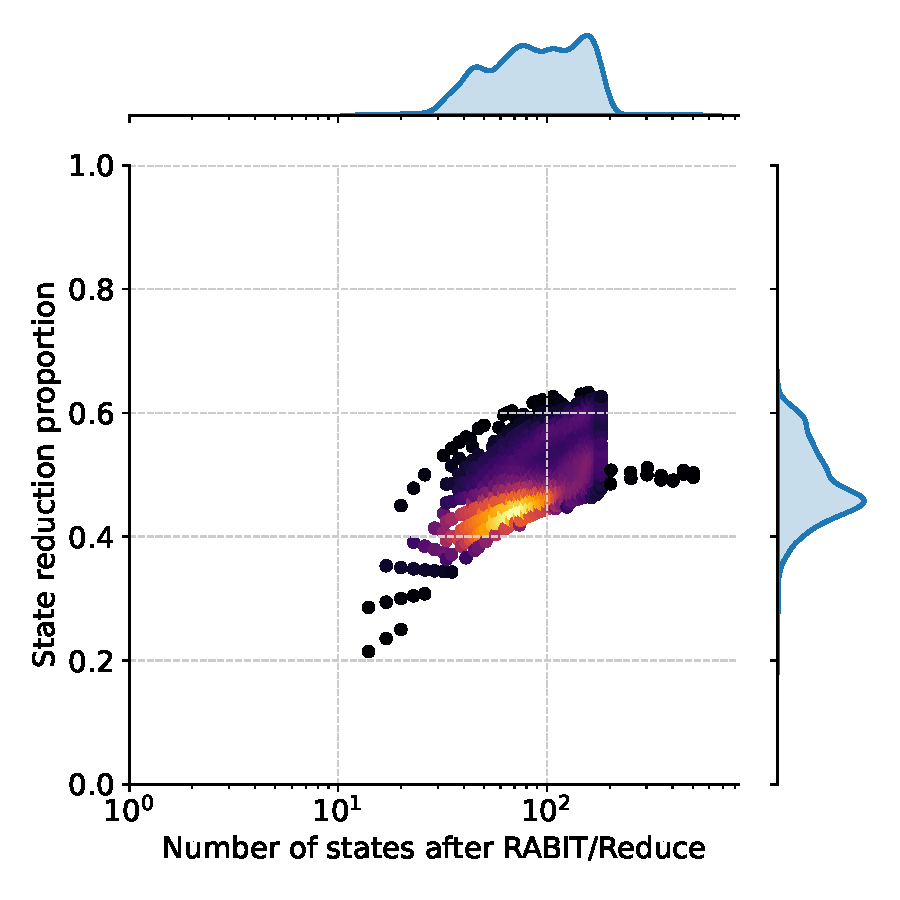
\includegraphics[width=1.1\textwidth]{img/intersect-all-states.pdf}

      \column{0.25\textwidth}
        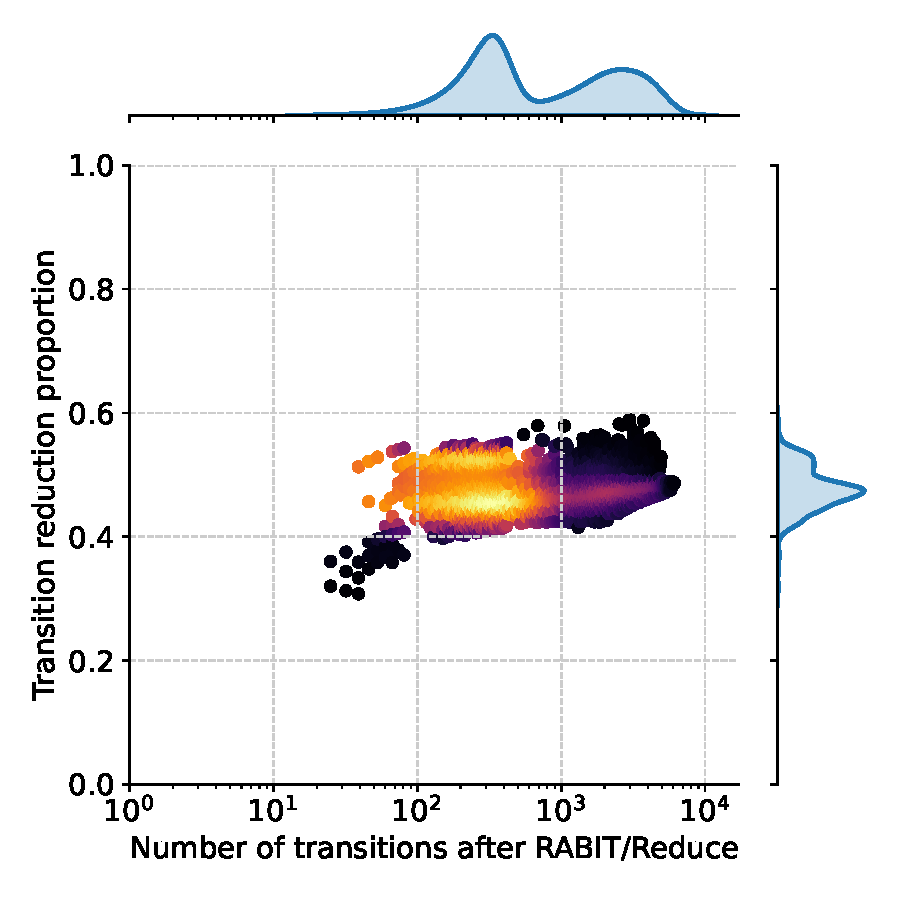
\includegraphics[width=1.1\textwidth]{img/intersect-all-trans.pdf}
    \end{columns}
  }

  \uncover<2->{
    \begin{columns}
      \column{0.5\textwidth}
        \emph{\textbf{Email Validations}}
        \begin{itemize}
          \item Total of \emph{362 automata}
          \item Max: 289 states and 10,333 transitions
          \item Average \emph{state reduction}: $29\%$
          \item Average \emph{transition reduction}: $28.6\%$
        \end{itemize}

      \column{0.25\textwidth}
        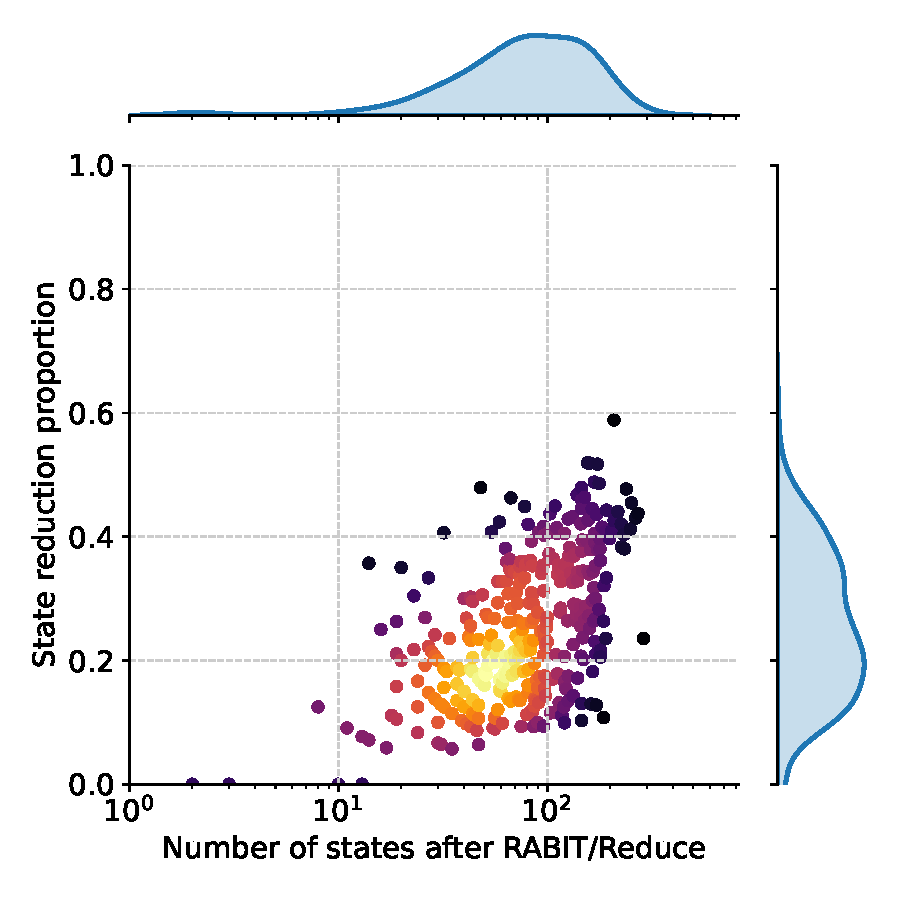
\includegraphics[width=1.1\textwidth]{img/emails-states.pdf}

      \column{0.25\textwidth}
      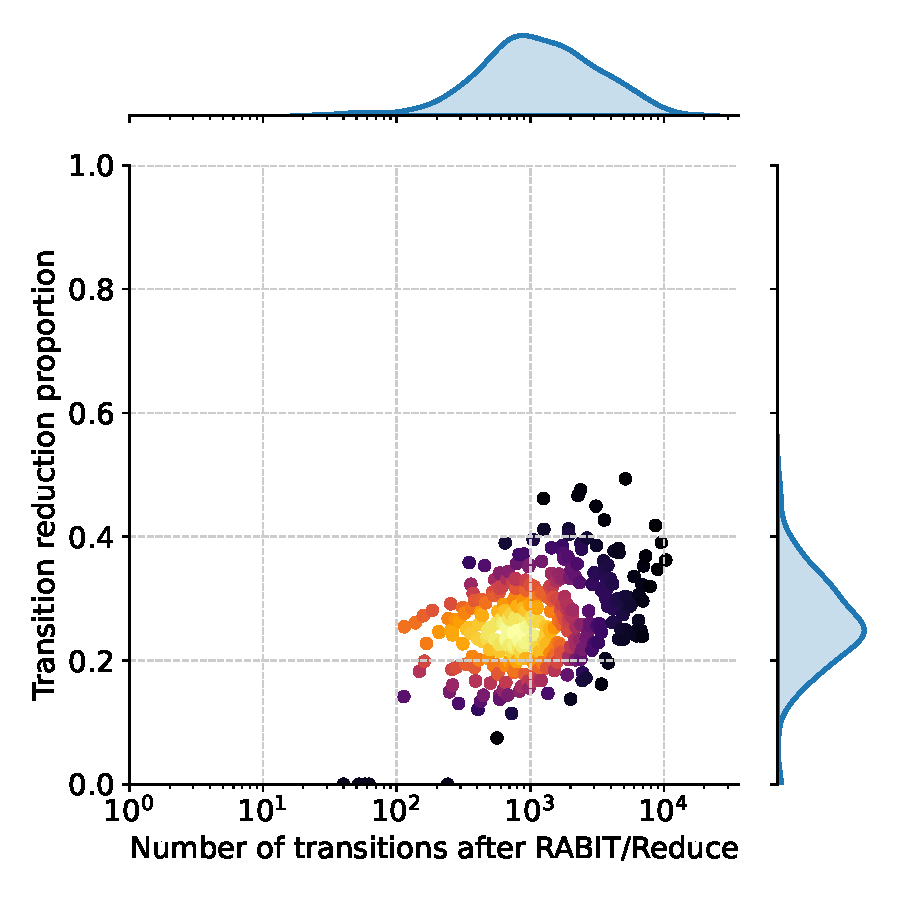
\includegraphics[width=1.1\textwidth]{img/emails-trans.pdf}
    \end{columns}
  }
\end{frame}


%%%%%%%%%%%%%%%%%%%%%%%%%%%%%%%%%%%%%%%%%%%%%%%%%%%%%%%%%%%%%%%%%%%%%%%%%
%%%%%%%%%%%%%%%%%%%%%%%%%%%%%%%%%%%%%%%%%%%%%%%%%%%%%%%%%%%%%%%%%%%%%%%%%
%%%%%%%%%%%%%%%%%%%%%%%%%%%%%%%%%%%%%%%%%%%%%%%%%%%%%%%%%%%%%%%%%%%%%%%%%
% Experimental Results - Snort (Network Filtering)
%%%%%%%%%%%%%%%%%%%%%%%%%%%%%%%%%%%%%%%%%%%%%%%%%%%%%%%%%%%%%%%%%%%%%%%%%
%%%%%%%%%%%%%%%%%%%%%%%%%%%%%%%%%%%%%%%%%%%%%%%%%%%%%%%%%%%%%%%%%%%%%%%%%
%%%%%%%%%%%%%%%%%%%%%%%%%%%%%%%%%%%%%%%%%%%%%%%%%%%%%%%%%%%%%%%%%%%%%%%%%
\begin{frame}
  \frametitle{Experimental Results - Snort (Network Filtering)}
    \begin{itemize}
      \item Total of \emph{3,616 regular expressions} from \emph{seven families} of Snort rules.
      \item Each automaton represents a \emph{union of regular expressions} from one family.
      \item The table illustrates the further minimization achieved by utilizing procedures, following the initial automaton reduction using the Rabit/Reduce tool, which employs state merging and transition pruning.\justifying
    \end{itemize}

    \blfootnote{\scriptsize$Q_{Proc} + \Gamma_{Proc}$: Number of states and stack symbols after procedure mapping.}
    \blfootnote{\scriptsize$\Gamma^{red}_{Proc}$: Number of stack symbols after stack alphabet reduction.}

    \vspace*{0.8em}

    \begin{centering}
      \hspace*{-1.75ex}
      \footnotesize
        \begin{tabular}{c|rr|rr|crrrc}
          Snort rules & \multicolumn{1}{c}{$Q_{in}$} & \multicolumn{1}{c|}{$\delta_{in}$} & \multicolumn{1}{c}{$Q_{RAB}$} & \multicolumn{1}{c|}{$\delta_{RAB}$} & \multicolumn{2}{c}{$Q_{Proc} + \Gamma_{Proc}$} & \multicolumn{2}{c}{$\delta_{Proc}$}& \multicolumn{1}{c}{$\Gamma^{red}_{Proc}$}\\
          \specialrule{.1em}{.05em}{.05em}
          p2p              & \hspace*{0.5em}33\hspace*{0.5em} &  1,090\hspace*{0.5em}   &\hspace*{0.5em} 32\hspace*{0.5em}   & 1,084\hspace*{0.5em}  & 25+6                   & (-3.1\%) & \hspace*{0.5em}570    & (-47.4\%) & 2\\
          worm             & \hspace*{0.5em}50\hspace*{0.5em} &  3,880\hspace*{0.5em}   &\hspace*{0.5em} 34\hspace*{0.5em}     & 290\hspace*{0.5em}    & 24+8                  & (-5.9\%)& \hspace*{0.5em}284    & (-2.1\%) & 2\\
          shellcode        & \hspace*{0.5em}162\hspace*{0.5em} & 3,328\hspace*{0.5em}   &\hspace*{0.5em} 56\hspace*{0.5em}     & 579\hspace*{0.5em}    & 48+2                 & (-10.7\%) & \hspace*{0.5em}486    & (-16.1\%) & 2\\
          \rowcolor{yellow}mysql            & \hspace*{0.5em}235\hspace*{0.5em} & 30,052\hspace*{0.5em} & \hspace*{0.5em} 91\hspace*{0.5em}  & 14,430\hspace*{0.5em} & 45+18\hspace*{-0.5em}   & (-30.8\%) & \hspace*{0.5em}7,142  & (-50.5\%) & 5\\
          chat             & \hspace*{0.5em}408\hspace*{0.5em} & 23,937\hspace*{0.5em} & \hspace*{0.5em}113\hspace*{0.5em}   & 1,367\hspace*{0.5em}  & 71+25\hspace*{-0.5em}  & (-15.0\%) & \hspace*{0.5em}1,058  & (-22.6\%) & 3\\
          \rowcolor{yellow}specific-threats & \hspace*{0.5em}459\hspace*{0.5em} & 57,292\hspace*{0.5em} & \hspace*{0.5em}236\hspace*{0.5em}  & 31,935\hspace*{0.5em} & 99+32\hspace*{-0.5em}   & (-44.5\%) & \hspace*{0.5em}12,680 & (-60.3\%) & 6\\
          telnet           & \hspace*{0.5em}829\hspace*{0.5em} & 7,070\hspace*{0.5em}  & \hspace*{0.5em}309\hspace*{0.5em}   & 2,898\hspace*{0.5em}  & 155+82                 & (-23.3\%) & \hspace*{0.5em}2,164  & (-25.3\%) & 4\\
        \end{tabular}
    \end{centering}
\end{frame}


\begin{frame}
  \frametitle{Future Work}
  \begin{columns}
    \column{0.62\textwidth}
    \vspace*{2em}
    \begin{itemize}
      \item Investigate the impact of the stack on the performance of automata operations.\justifying
      \item Incorporate automata with a stack in hardware\break to scan high-speed networks.\justifying
      \item Improve the detection of similar substructures.\justifying
      \item Effectively utilize a greater stack depth.\justifying
    \end{itemize}

    \vspace*{3.5em}

    \uncover<2->{
    \hspace*{6ex}\emph{\textbf{\Large{Thank you for your attention!}}}
    }
    \column{0.3\textwidth}
    
\includegraphics[width=1\textwidth]{img/todo2.jpg}
    \vspace*{-11em}
  \end{columns}
\end{frame}

%%%%%%%%%%%%%%%%%%%%%%%%%%%%%%%%%%%%%%%%%%%%%%%%%%%%%%%%%%%%%%%%%%%%%%%%
%%%%%%%%%%%%%%%%%%%%%%%%%%%%%%%%%%%%%%%%%%%%%%%%%%%%%%%%%%%%%%%%%%%%%%%%
%%%%%%%%%%%%%%%%%%%%%%%%%%%%%%%%%%%%%%%%%%%%%%%%%%%%%%%%%%%%%%%%%%%%%%%%
% Appendix
%%%%%%%%%%%%%%%%%%%%%%%%%%%%%%%%%%%%%%%%%%%%%%%%%%%%%%%%%%%%%%%%%%%%%%%%
%%%%%%%%%%%%%%%%%%%%%%%%%%%%%%%%%%%%%%%%%%%%%%%%%%%%%%%%%%%%%%%%%%%%%%%%
%%%%%%%%%%%%%%%%%%%%%%%%%%%%%%%%%%%%%%%%%%%%%%%%%%%%%%%%%%%%%%%%%%%%%%%%
\appendix{}
\begin{frame}
  \frametitle{Reduce or Not to Reduce?}
  \begin{itemize}
    \item Why is the size of the stack alphabet reported before reduction?
  \end{itemize}

  \vspace*{1em}

  \uncover<2->{
    \begin{figure}
      \centering
      \begin{tikzpicture}[scale=0.6, node distance=2cm, every node/.style={font=\footnotesize, scale=0.6}]
        \node[state, initial] (q0) {$q_0$};
        \node[state, right of=q0] (q1) {$q_1$};
        \node[state, right of=q1] (q2) {$q_2$};
        \node[state, right of=q2] (q3) {$q_3$};
        \node[state, right of=q3] (q4) {$q_4$};
        \node[state, right of=q4] (q5) {$q_5$};
        \node[state, accepting, right of=q5] (q6) {$q_6$};

        \path[->]
                (q0) edge[above] node{$a$} (q1)
                (q1) edge[above] node{$b$} (q2)
                (q2) edge[above] node{$c$} (q3)
                (q3) edge[above] node{$d$} (q4)
                (q4) edge[above] node{$e$} (q5)
                (q5) edge[above] node{$f$} (q6);
      \end{tikzpicture}
    \end{figure}
  }

  \begin{columns}
    \uncover<3->{
      \column{0.5\textwidth}
        \begin{figure}
          \centering
          \begin{tikzpicture}[scale=0.8, node distance=3cm, every node/.style={font=\footnotesize, scale=0.8}]
            \node[rectangular state, initial, accepting, initial text=$q_0$] (q0) {$even$};
            \node[rectangular state, right of=q0] (q1) {$odd$};

            \path[->]
                    (q0) edge[below, bend right=10] node{$\begin{aligned}
                                                            &a,q_0/q_1\\[-1mm]
                                                            &c,q_2/q_3\\[-1mm]
                                                            &e,q_4/q_5
                                                        \end{aligned}$} (q1)
                    (q1) edge[above, bend right=10] node{$\begin{aligned}
                                                            &b,q_1/q_2\\[-1mm]
                                                            &d,q_3/q_4\\[-1mm]
                                                            &\hspace*{0.5ex}f,q_5/\varepsilon
                                                        \end{aligned}$} (q0);

          \end{tikzpicture}
        \end{figure}
    }

    \uncover<4->{
      \column{0.5\textwidth}
        \begin{figure}
          \centering
          \begin{tikzpicture}[scale=0.8, node distance=3cm, every node/.style={font=\footnotesize, scale=0.8}]
            \node[rectangular state, initial, accepting, initial text=$q_0$] (q0) {$even$};
            \node[rectangular state, right of=q0] (q1) {$odd$};

            \path[->]
                    (q0) edge[below, bend right=10] node{$\begin{aligned}
                                                            &a,q_{0,1}/q_{0,1}\\[-1mm]
                                                            &c,q_{2,3}/q_{2,3}\\[-1mm]
                                                            &e,q_{4,5}/q_{4,5}
                                                        \end{aligned}$} (q1)
                    (q1) edge[above, bend right=10] node{$\begin{aligned}
                                                            &b,q_{0,1}/q_{2,3}\\[-1mm]
                                                            &d,q_{2,3}/q_{4,5}\\[-1mm]
                                                            &\hspace*{0.5ex}f,q_{4,5}/\varepsilon
                                                        \end{aligned}$} (q0);

          \end{tikzpicture}
        \end{figure}
    }
  \end{columns}

  \begin{columns}
    \hspace*{1.7cm}
    \uncover<3->{
      \column{0.55\textwidth}
        \scriptsize
        \begin{itemize}
          \item 2 states\vspace*{-0.8mm}
          \item 6 stack symbols\vspace*{-0.8mm}
          \item \emph{no reduction}
        \end{itemize}
    }
    \uncover<4->{
      \column{0.5\textwidth}
      \scriptsize
      \begin{itemize}
        \item 2 states\vspace*{-0.8mm}
        \item 3 stack symbols\vspace*{-0.8mm}
        \item \emph{28.6\% reduction} (Or is it?)
      \end{itemize}
    }
  \end{columns}

\end{frame}

%%%%%%%%%%%%%%%%%%%%%%%%%%%%%%%%%%%%%%%%%%%%%%%%%%%%%%%%%%%%%%%%%%%%%%%%%
%%%%%%%%%%%%%%%%%%%%%%%%%%%%%%%%%%%%%%%%%%%%%%%%%%%%%%%%%%%%%%%%%%%%%%%%%
%%%%%%%%%%%%%%%%%%%%%%%%%%%%%%%%%%%%%%%%%%%%%%%%%%%%%%%%%%%%%%%%%%%%%%%%%
% Appendix - Opponent's Questions
%%%%%%%%%%%%%%%%%%%%%%%%%%%%%%%%%%%%%%%%%%%%%%%%%%%%%%%%%%%%%%%%%%%%%%%%%
%%%%%%%%%%%%%%%%%%%%%%%%%%%%%%%%%%%%%%%%%%%%%%%%%%%%%%%%%%%%%%%%%%%%%%%%%
%%%%%%%%%%%%%%%%%%%%%%%%%%%%%%%%%%%%%%%%%%%%%%%%%%%%%%%%%%%%%%%%%%%%%%%%%
% \begin{frame}
%   \frametitle{Opponent's Questions}
%   \vspace*{-3.55em}
%   \begin{itemize}
%     \item Jaké jsou Vaše publikační plány související s touto prací?
%   \end{itemize}

%   \vspace*{4.5em}

%   \uncover<2->{
%     \begin{centering}
%       \epigraph{\textit{...plánujeme publikovat na konferenci typu FM, TACAS, a pravděpodobně navážeme aplikací práce v akceleraci rozpoznávání regulárních vzorů pomocí FPGA v monitorování síťového provozu.}\justifying}{--- doc. Mgr. Lukáš Holík, Ph.D., \textit{"Supervisor assessment of Master's Thesis"}}
%     \end{centering}
%   }

% \end{frame}
